\documentclass[11pt, a4paper]{article}
\usepackage[margin=1in]{geometry}

\usepackage{lmodern}
\fontfamily{lmdh}\selectfont

\usepackage{graphicx}
\graphicspath{{../}}

\usepackage{titlesec}
\titleformat*{\section}{\large\bfseries}

\usepackage{caption}
\captionsetup[figure]{font={small, bf}}

\usepackage{subcaption}

\usepackage[style=authoryear-ibid,backend=biber]{biblatex}
\renewcommand*{\nameyeardelim}{\addcomma\space}
\addbibresource{ag_bib.bib}

\usepackage{verbatim}

\title{\large\bfseries Classification and Pricing of Farmed Abalone}
\author{\normalsize A. Gill}
\date{\small \today}

\begin{document}
    
    \maketitle

    \section*{Introduction}    
      
    An enquiry has been made as to the potential use of lightweight software, installed on diving equipment, to help abalone farmers to quickly assess whether an abalone should be harvested or left in the water. There are two main parameters in making such an assessment:

    \begin{itemize}
        \item \textbf{Sex.} Female abalone are more valuable, because their eggs are used to reduce water toxicity \parencite{atlantic}. On the other hand, mature males may be sought, to ensure that enough females are left to allow reproduction to occur.
        \item \textbf{Age.} Infant abalone (that have not yet reached sexual maturity) should be avoided, because their small size yields less meat. In addition, they should be allowed to reach maturity and contribute to reproduction.
    \end{itemize} 

    The aim is to use non-intrusive measurements - length, diameter and height - to predict an abalone's sex and infancy status, as well as estimate its weight (and thus market value), allowing farmers to return rejected abalone to the water without having harmed them. Modelling techniques shall be applied to data from previously harvested abalone, to develop predictive tools for this purpose.

    \section{Exploratory Analysis}

    Data on more than 4000 harvested abalone have been supplied. The dataset includes the following columns (variables):

    \begin{itemize}
        \item Sex
        \item Length, diameter and height
        \item Whole, shucked, viscera and shell weights
        \item Number of rings on the shell (an indicator of age)
    \end{itemize}

    The data have been checked for missing or impossible values. No entries are missing, but two abalone have a recorded height of 0, a physical impossibility. These two rows have been removed.

    The modelling techniques to be used depend on the supplied data meeting certain conditions:

    \begin{itemize}
        \item \textbf{Normality.} When the probability of each value occurring is graphed against the value itself, the curve (known as a density plot) should form the classical bell shape expected of ``normal'' data.
        \item \textbf{Linearity.} The relationship between each pair of variables should be linear (or close to a straight line).
        \item \textbf{Homoscedasticity.} The variation (spread) in one variable should remain the same, regardless of the value of another variable. 
    \end{itemize}

    \subsection{Normality}

    The density plots for all the numerical variables are shown in Figure \ref{density}.

    \begin{figure}[ht]
        \centering
        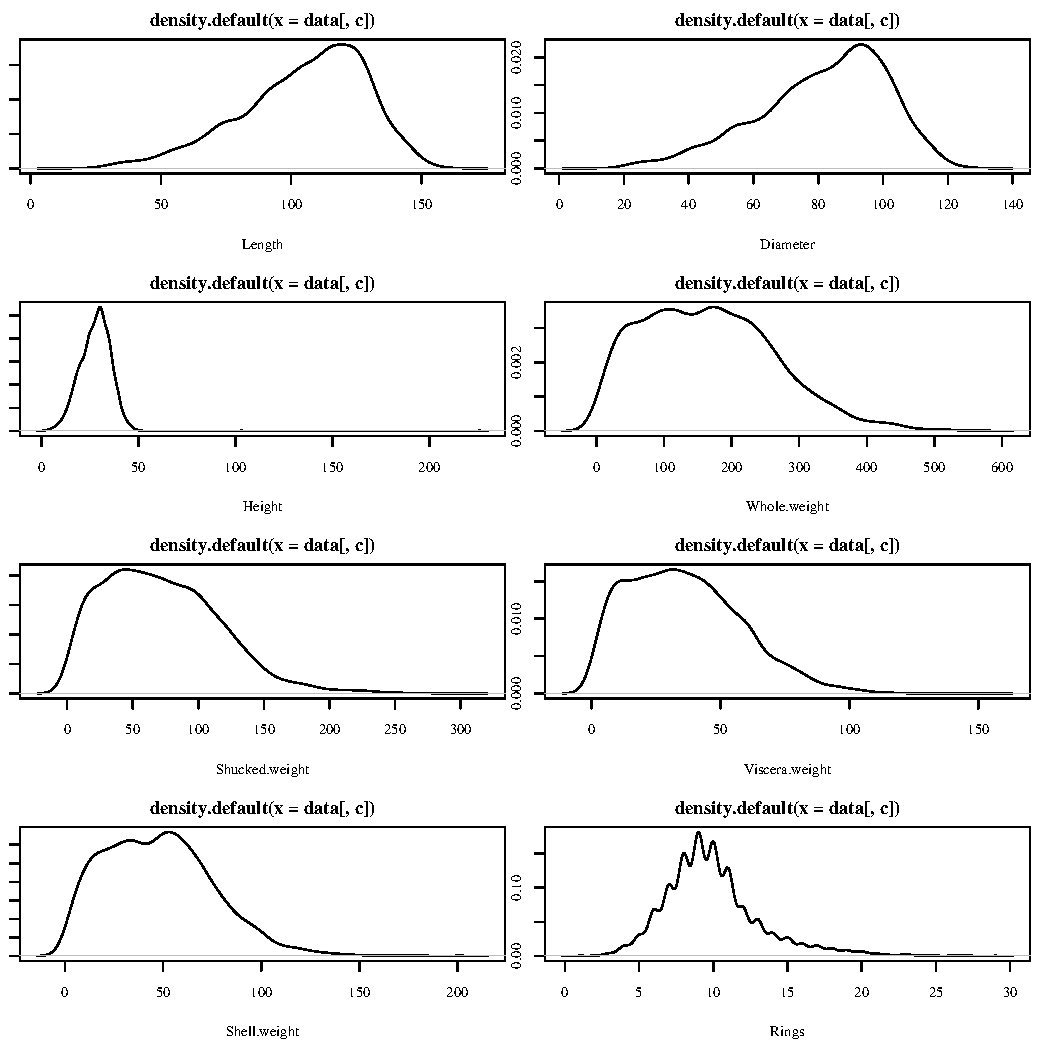
\includegraphics[width=\textwidth]{1.4.pdf}
        \caption{Density Plots}
        \label{density}
    \end{figure}

    All of the variables are skewed; that is, the bell curve is stretched either left or right, meaning the data may not be sufficiently ``normal''. This can be repaired, to some extent, by transforming the data i.e. mathematically altering the values to force them into a more symmetrical shape.

    \subsection{Linearity and Homoscedasticity}

    These two requirements can be checked by plotting pairs of the variables against one another, as shown in Figure \ref{pairs}. The following observations can be made:

    \begin{itemize}
        \item The relationships between all the weight variables, and the length and diameter, are non-linear. 
        \item As the number of rings increases, the variation (spread) in all the other variables (except height) also increases. However, because the counting of rings is an intrusive process, this variable is to be excluded from the modelling, and this failure of homoscedasticity can be ignored.
        \item The slightly oval shape of the plots pairing the four weights suggests that these variables are normally distributed. Examining Figure \ref{density} confirms that the four weight variables are the most ``normal'', with low kurtosis (pointiness) but some skew to the right.
    \end{itemize}

    \begin{figure}[ht]
        \centering
        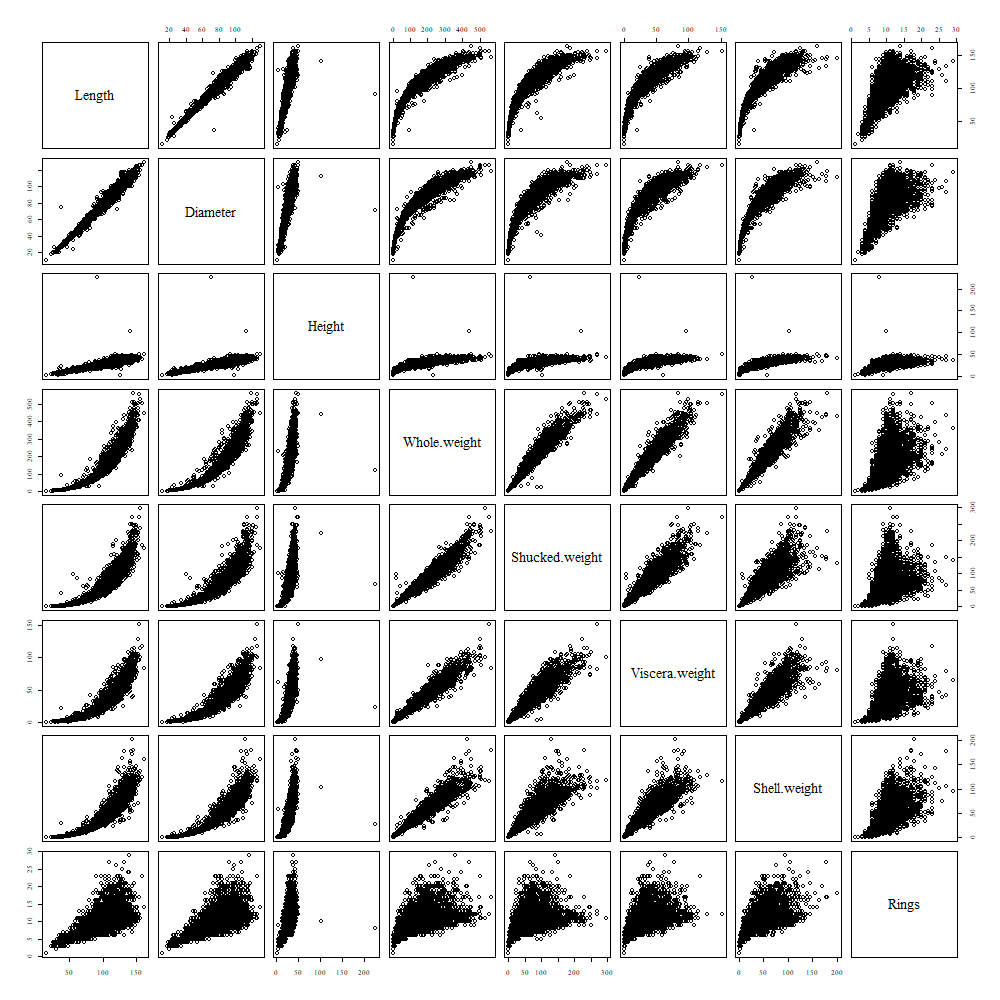
\includegraphics[width=\textwidth]{1.3.png}
        \caption{Scatter Plots of Variable Pairs}
        \label{pairs}
    \end{figure}

    \subsection{Data Correction}

    As mentioned earlier, the variables can be transformed to normalise them. A transformation can be as simple as taking the square root or logarithm of every value in the data column. 

    Transformations have the additional benefit of pulling outliers (extreme values) in towards the bell, so that they are no longer considered extreme. Then, any remaining outliers may be removed from the dataset. They can also help to improve the linearity of the relationships between the variables.

    Table \ref{outliers} shows that most outliers have been successfully addressed by the transformations, leaving only a small number to be removed from the dataset (with the exception of height). Figure \ref{density.t} illustrates a substantial improvement in every variable, after applying a transformation and removing the remaining outliers. 
    
    \begin{table}[ht]
        \centering
        \begin{tabular}{|l|c|c|}
            \hline
            Variable&Initial Outliers&Remaining Outliers \\
            \hline
            Length & 49 & 8 \\
            Diameter & 59 & 9 \\
            Height & 27 & 156 \\
            Whole weight & 30 & 1 \\
            Shucked weight & 48 & 3 \\
            Viscera weight & 26 & 2 \\
            Shell weight & 35 & 8 \\
            Rings & 278 & 268 \\
            \hline
        \end{tabular}
        \caption{Outliers Before and After Transformations}
        \label{outliers}
    \end{table}

    \begin{figure}[ht]
        \centering
        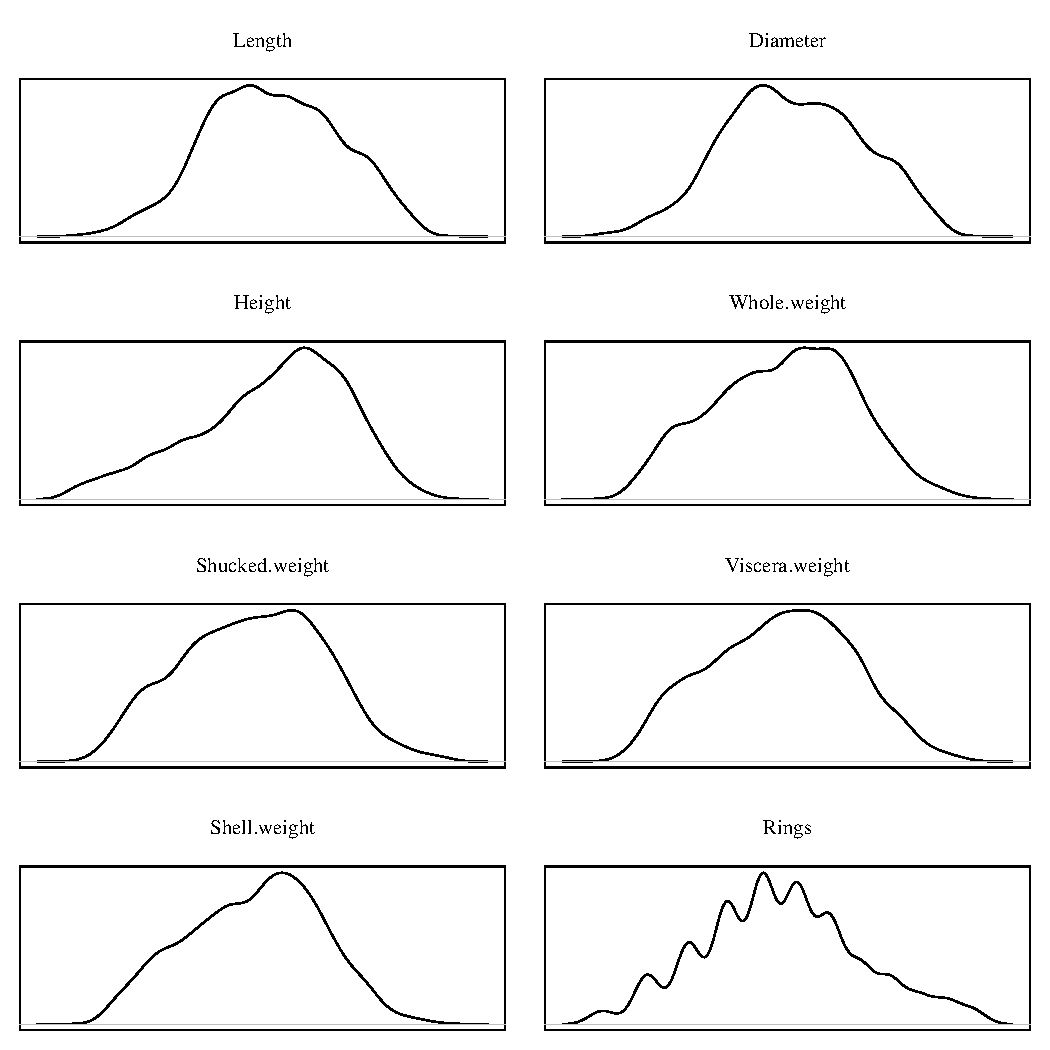
\includegraphics[width=\textwidth]{1.7.pdf}
        \caption{Density Plots After Transformations and Removal of Outliers}
        \label{density.t}
    \end{figure}

    Having confirmed, through measurements of skewness and kurtosis, that the variables are now much closer to ``normal'' than they were before, data modelling to predict sex and infancy status can now proceed.

    \section{Predicting Sex and Infancy}

    The supplied data have been fed into two machine learning algorithms in order to develop a ``classifier'' that labels an abalone an infant, female or male, based on non-intrusive inputs (length, diameter and height). 

    The first algorithm involves \textbf{discriminant analysis}; the second involves a \textbf{support vector machine}. Detailed explanations for these algorithms can be found in XXXX and XXXX. 

    \subsection{Three-Way Classifier}

    Two variants of discriminant analysis have been attempted; LDA (linear discriminant analysis) and QDA (quadratic discriminant analysis). LDA assumes that the variance (spread) of values for all variables is the same. However, testing has confirmed that this is not the case for abalone. Nevertheless, LDA may still produce good results and is thus worth considering.

    In addition to LDA and QDA, two support vector machines have been attempted; linear and radial. Table \ref{three-way} reports the accuracy for each of the attempted algorithms.

    \begin{table}[ht]
        \centering
        \begin{tabular}{|l|c|}
            \hline
            Model & Accuracy \% \\
            \hline
            QDA & 0.5050 \\
            LDA & 0.5153 \\
            SVM linear & 0.5147 \\
            SVM radial & 0.5168 \\
            \hline
        \end{tabular}
        \caption{Accuracy of Three-Way Classifiers}
        \label{three-way}
    \end{table}

    The overall accuracy for all models is poor, but is slightly better for SVM. Table \ref{svm-acc} shows the accuracy of the two SVM models by class (infant, female, male).

    \begin{table}[ht]
        \centering
        \begin{tabular}{|l|c|c|}
            \hline
            Class & Accuracy (Linear) \% & Accuracy (Radial) \% \\
            \hline
            Infant & 0.7206 & 0.7121 \\
            Female & 0 & 0.0025 \\
            Male & 0.7820 & 0.7926 \\
            \hline
        \end{tabular}
        \caption{Accuracy of Three-Way Classifiers}
        \label{svm-acc}
    \end{table}

    Nearly all of the female abalone are classified incorrectly by these models. By contrast, their accuracy is acceptable (above 70\%) for infants, and approaching good (nearly 80\%) for males. In order to understand this phenomenan, the three input variables can be summarised as boxplots, as shown in Figure \ref{boxplots}.

    \begin{figure}[ht]
        \centering
        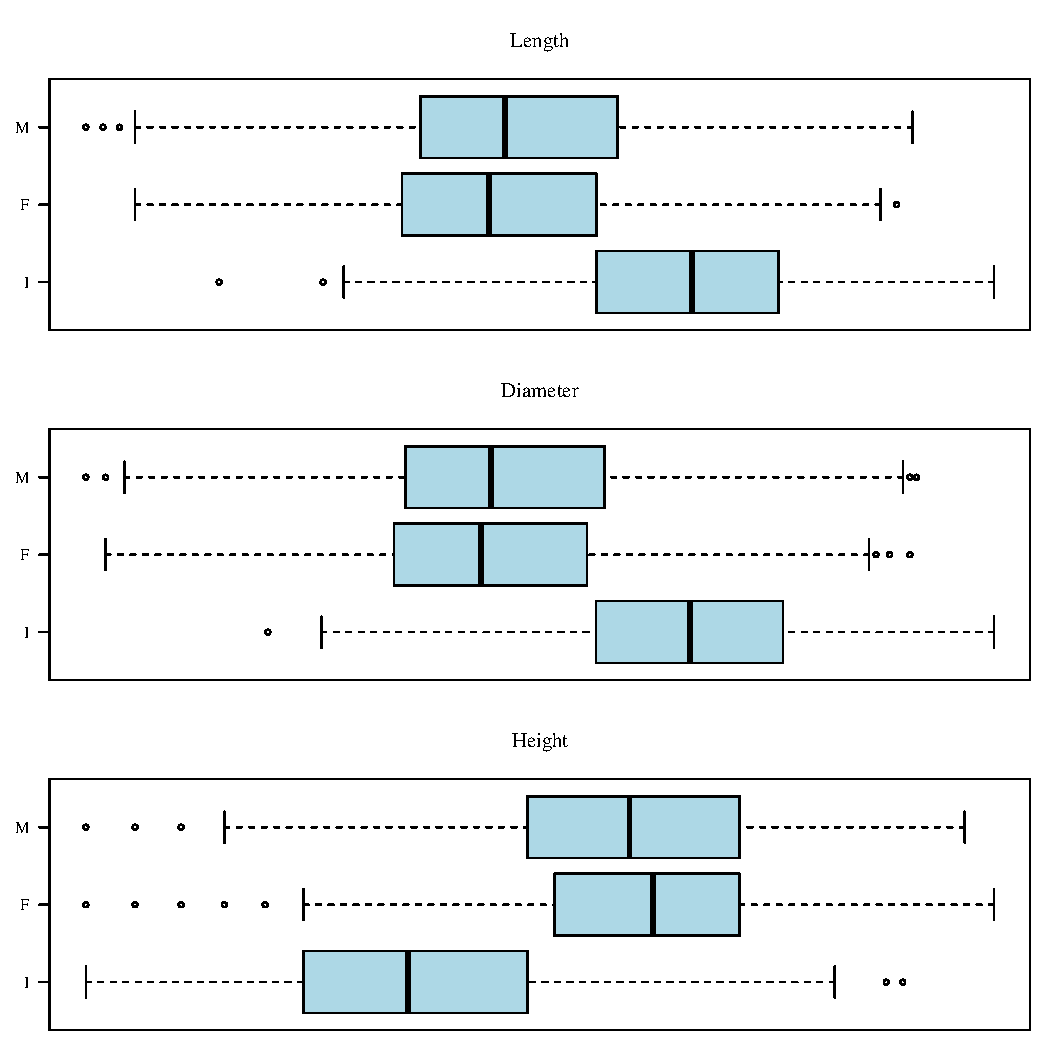
\includegraphics[width=\textwidth]{2.4.pdf}
        \caption{Input Variables by Sex Class}
        \label{boxplots}
    \end{figure}

    The boxplots show that the values of length, diameter and height for males and females are considerably overlapped, while the values for infants are substantially separated from the other classes. This explains why the models are unable to differentiate between males and females.

    Because of this, \textbf{none} of the models is suitable as a three-way classifier, although the best-performing model, SVM with a radial kernel, may be used to identify infants and males.

    \subsection{Binary Classifiers}

    Having failed to specify a classifier suitable for labelling infants, females and males, binary classifiers have been attempted, to differentiate between:

    \begin{itemize}
        \item Infants and non-infants (to avoid harvesting infant abalone)
        \item Females and non-females (to selectively harvest females for increased profits)
        \item Males and non-males (to selectively harvest males to preserve female populations)
    \end{itemize}

    A performance summary for the best models in these scenarios is given in Table \ref{binary}. While it appears that all three models perform reasonably well, closer inspection confirms otherwise. The following are the observations from the \textbf{confusion matrix} shown in Table \ref{cms}:

    \begin{itemize}
        \item \textbf{I vs Not I}: Very good at identifying non-infants, but poor at identifying infants.
        \item \textbf{F vs Not F}: Classifies nearly all abalone as non-female, regardless of true sex.
        \item \textbf{M vs Not M}: Classifies nearly all abalone as non-male, regardless of true sex.
    \end{itemize}  

    \begin{table}[ht]
        \centering
        \begin{tabular}{|l|l|c|}
            \hline
            Classifier  & Best Model    & Accuracy \% \\
            \hline
            I vs Not I  & SVM radial    & 0.7950 \\
            F vs Not F  & SVM radial    & 0.6926 \\
            M vs Not M  & SVM radial    & 0.6824 \\
            \hline
        \end{tabular}
        \caption{Accuracy of Three-Way Classifiers}
        \label{binary}
    \end{table}

    \begin{table}
        \centering
        \begin{tabular}{|l|c|c|}
            \hline
                            & Predicted & Predicted Not \\
            \hline
            Actual I        & 675       & 506 \\
            Actual Not I    & 273       & 2346 \\
            \hline
            Actual F        & 84        & 1122 \\
            Actual Not F    & 46        & 2548 \\
            \hline
            Actual M        & 1         & 1412 \\
            Actual Not M    & 0         & 2387 \\
            \hline           
        \end{tabular}
        \caption{Confusion Matrix for Binary Classifiers}
        \label{cms}
    \end{table}

    Therefore, it is recommended that a binary classifier for infants and non-infants \textbf{only} be used to positively identify non-infants, not for identifying infants. In addition, it is recommended that a binary classifier \textbf{not} be used at all for females and non-females, and males and non-males.

    Unfortunately, this means that the objective to use non-intrusive measurements to predict the sex of abalone cannot be met, because males and females are not differentiable by their physical proportions; rather, the best  method of determining sex is to examine the colour of the abalone's underside (XXXX). 

    \section{Estimating Price}

    Depending on species and habitat, smaller abalone tend to be younger in age, and larger abalone tend to be older. Therefore, by returning smaller abalone to the water and allowing them to mature and reproduce, farmers can ensure sustainability of abalone populations, while maximising their own profits by selectively harvesting larger (older) abalone with more meat.

    To this end, an algorithm has been developed by which a farmer can quickly predict the shucked and viscera weights of an abalone, based only on its measurements, and thus estimate the market value.

    Using the supplied data on previously harvested abalone, a \textbf{multiple linear regression} (MLR) model has been fed the measurements for length, diameter and height. The resulting equations that allow prediction of the shucked and viscera weights are:

    



\end{document}

